\hypertarget{configure-able-methods}{%
\section{Configure-able methods}\label{configure-able-methods}}

This chapter covers the initial inquiry of my research, and the
coalescing together of crip theory and critical access with that of
Feminist Science and Technologies Studies (STS). In this chapter I
wiggle together these research tables to make room for Configure-able
methods to emerged from this research. This inquiry does feel a little
like a second literature review in some places, and this is because I
wanted to centre my approach from Crip studies within
\href{../../01_Disability_justice_and_life_affirmation_flipping_the_table/01_Disability\%20justice\%20and\%20life\%20affirmation\%20flipping\%20the\%20table.md}{01\_Disability
justice and life affirmation flipping the table} and in this chapter
coalesce this with more of an accessible understanding of Feminist STS
methods. To emerge this methodology I first trace a genealogy of
configuration from its routes in figure and figuring (Lury et al., 2022)
to that of Suchman's definition of Configuration (2012). I then
disorient it with an -able and critiques of critical access (Hamraie,
2017) and crip studies (Kafer, 2013) to question how configuration can
be shaped when brought into contact with the dispersed and indeterminate
practices, bodies and expertise of access in action. In reflection of my
experiences configuring access for the \emph{Configure-Able
Infrastructures} workshops I ran at NEoN I offer how critical access as
a practice and method centres indeterminate localities and imperfect
improvisations instead of the determined curative hard plans which
forcefully shapes bodies and systems. With both Hamraie and Kafer, I
question what the problem is within configurations, cripping it from
isolated individualised issues to relational constraints of centralised
plans. With this disorientation I also question how sedimented roles of
user/designer/expert, prescribed/prescriber, or ethnographer/community
can be reconfigured from the sites of impact and frictions within
collective practices.

\hypertarget{figuring-out-a-genealogy-of-configuration}{%
\subsection{Figuring out a Genealogy of
Configuration}\label{figuring-out-a-genealogy-of-configuration}}

Like much of the work I am engaged with, Configure-able methods are an
attempt to enact methods, practices and their terms so that they can be
accessible to and improvised by different positions. The term
configure-able, for me gives an initial proposition of disorientation,
some sort of re-figuring of configurations through a crip critique of
critical access, but also room to configure configurations. In
\href{../../01_Disability_justice_and_life_affirmation_flipping_the_table/01_Disability\%20justice\%20and\%20life\%20affirmation\%20flipping\%20the\%20table.md}{01\_Disability
justice and life affirmation flipping the table} I already covered in
great depth my understanding of the background of crip studies and its
hacking practices and abilities within technoscience as well as my
experiences of disability that informs this understanding in both
\href{../../01_Disability_justice_and_life_affirmation_flipping_the_table/sections/01.02.00_The_Crip_Table.md}{01.02.00\_The\_Crip\_Table}
and
\href{../../02_Crip-Tic_of_Vignettes/02_Crip-Tic_of_Vignettes.md}{02\_Crip-Tic\_of\_Vignettes}
sections. This definition here then focuses on the pre-intonation of
configure before the -able, the orientation before the turn, inflection
or retreat. Here I come to this table of configuration, approaching it
from this prior one of disability, and in doing so coalesce it closer.
In this dance I follow its roots as figures in motion, and so
(hopefully) an accessible definition of figures and configuration as an
axis that I can inflect and coalesce with critical access and crip
theory in the build up to the later
\href{04.02.02_Cripping\%20Configuration.md}{04.02.02\_Cripping
Configuration} section.

\hypertarget{figure}{%
\subsubsection{Figure}\label{figure}}

To define figure, I start by working closely with Celia Lury et. al's
already fairly accessible definition (2022). In the intro chapter to
their \emph{Figure Concept and Method} book they define two propositions
of figure, one as a noun and one as a verb. The difference in the two is
key, as I will share, as it takes us from passive and inherited
determined figures, and stories of a world, to being able to figure out
our own stories and relations with each other and technologies.

\hypertarget{as-a-noun-figure}{%
\paragraph{As a noun, Figure}\label{as-a-noun-figure}}

To define figure as a noun, they first build up from Erich Auerbach's
(2013) tracing of its etymology within ``Figura'' in Latin. Figura
developed from a constellation of technical Greek words that orient the
materiality of things and plays between plasticity and form within their
shaping. Auerbach raises the tension within Figura which came about to
think through this delineation of both the material and conceptual
elements of an object. In a sense this meant that within western
discourse Figura, or later figures, became a place to pivot or orient
our understanding of the material through the conceptual. Figures are
sedimented into christian doctrine, where stained in glass they can be
understood as a way of forming futures from pasts\footnote{``The Old
  Testament ``pre- figures'' the New Testament, past and future are
  symbiotically shaped in, and indeed incarnated by, typology: Word made
  flesh" (Lury, Viney, and Wark 2022, 2)}, making prophesy from historic
fables. Quoting Hayden White, Lury et al.~states that the use of figures
to represent this exchange is ``Western culture's unique achievement of
identifying reality as history''(1999, 96). In this motion of
prefiguring, Auerbach understands a flow of figuring that
deterministically moves into set configurations of material practices
and the limited scoping of their possibility.

When brought into the fields of social and political studies Figures are
used in multiple ways. Lury et al.~highlights Norbert Elias (1987) as a
sociologist who focuses on the relationality and interdependence of
persons and the ways this can figure their configuration. In his work he
states it is the role of a social scientist to understand how these
configurations bind them to their subject another (ibid., 79). This
understanding of figures as relational practices forms the base for
figurational sociology. In these figurational practices we start to
understand that figures are not determined prototypes, but act as
stories in motion, plastic and performable. Lury runs through a few of
these performances of figures in relation, moving from an isolated and
disinterested flâneur by Charles Baudelaire through to Walter Benjamin's
crowd (2003). In doing this she not only shares the plasticity of the
figure, but also how in their relationality they are lived through.

The final critique Lury et al.~(2022, 4) make of the figure as a noun is
of its western context, of the list of white men referenced to manifest
it here in writing. In the most part, they point out that within this
relational practice of the figure is a practice of differencing and
division\footnote{``the fig-ure of ``man'' figures who gets to be
  considered human by means of a series of constitutive exclusions
  (Mbembe 2017). Does one have to be male to count as ``man''? White?
  Western? Wealthy? Able-bodied?" (Lury, Viney, and Wark 2022, 4)}. To
examine this division further they take up Alexander G. Weheliye's
critique of ``racialisation'' (2014) as a crucial axis. With Weheliye
they question sedimented figures by moving from following what they
scope to questioning how they are scoped. Through this inversion of
their approach to figures it can be understood as a probing tool, one
for reflecting on and feeling out our means of producing knowledge.

Interestingly this movement of inverting the figure to understand its
maker also resonates with the move of the social model of disabilitie's
inversion of the medical model which I talk more about in the
\href{../../01_Disability_justice_and_life_affirmation_flipping_the_table/sections/01.02.01_PoliticalRelational_Model.md}{01.02.01\_PoliticalRelational\_Model}
entry. In this move the social model's inversion of sedimented power
relations and their practices, even though useful to understand certain
aspects of power, can in some ways miss the nuance of relations. With a
crip approach I look to trouble this by exploring how a figure can of
course be inverted, but also what other relations and practices can I
make room for when I choose to feel the frictions between figures and
their backgrounds.

\hypertarget{as-a-verb-figuring}{%
\paragraph{As a verb, Figuring}\label{as-a-verb-figuring}}

Figuring as a verb takes on the action of forming figures, of figuring
things out and of composing or computing figures. within this diversity
of forms and use of figure there is a focus on the tactility of thinking
when we are working through them. Taken as method figuring makes room to
apprehend the shape of something, of feeling out a figure, collating one
together, and making wiggle room for another one to join. In this
figuring out of space, much like with the noun, is this division of what
is brought into being a figure and what is backgrounded to contour that
figure. Lury et al.~approaches this with Edgar Rubin's psychological
research into perception (1958), where his depiction of figure and
ground are defined by the ``contour'' that runs between them. They give
the example of the ``Rubin vase''\footnote{````Rubin vase,'' which can
  be seen as a decorative vase on a dark background or two faces on a
  light background---reflects on its own conditions of emergence" (Lury,
  Viney, and Wark 2022, 6)}. With Ahmed I could similarly ask what
contingent approaches and practises do I rely upon, turning back to them
when feeling out contours of bodily-horizons, as I have not found
another path I yet desire, or another background to figure out from.
This is especially true within disability studies where the figure of
the crip is only just disobediently emerging into discourse of other
fields, and has always been kept in the background. With my crip
figuring out it is to make wiggle room around these sedimented norms for
this disabled figure to be contoured among, and with it the demands of
critical access and disobedient relational politics of crip theory.

\hypertarget{configuration}{%
\subsubsection{Configuration}\label{configuration}}

Configuration much like configure-able is an inflection, a changing in
tone, context and approach of figure which ``fixes'' it into a
generative materially entangled orientation. Lury et al.~(ibid., 8)
define configuring as a practice within complex systems design that
makes room to join diverse elements into arrangement, never final even
when ``stable''. It doesn't refer to the final arrangement of
components, but instead this practise of coalescing them together. Due
to configuring being this process of bringing figures into action, as
well as bringing the diverse elements of infrastructure together, it has
been taken up by Science Technology Studies (STS) as a cornerstone
critical methodology and mode of analysis. Lury et al.~here points to
Lucy Suchman's definition of Configuration to demonstrate how this
methodology can make room to inquire with ``{[}a{]}t once action and
effect''(2012, 49). Suchman's definition makes room to understand how
the stories that are told and the figures that are held in place produce
specific sedimented practices of ordering. In configuration as method
she makes room for a mode of analysis that can be an un/remaking through
material practises and their knowledges. Lury et al.~go on to trace
configuration through the work of D. N. Rodowick (2001), Michel
Foucault's notion of similitude(2020), as well as Donna Haraway's
``string figures''(1997) and her Cyborg Manifesto (1985), which I touch
on more in the
\href{../../01_Disability_justice_and_life_affirmation_flipping_the_table/sections/01.02.04_Cripping_Technoscience.md}{01.02.04\_Cripping\_Technoscience}
section. These movements by Lury et al.~in many ways orients towards
their understanding of Elizabeth Povinelli (2016) and Michelle Murphy
(2017) work as practices of forming figures ``equal to contemporary
political configurations''(Lury, Viney, and Wark 2022, 10).
Configure-Able Methods as I will go on to offer up, moves with these
approaches of forming counter figures, but also (un)fixes these
practices through impact centred design methods of critical access. Here
making room to form wiggle room through these counter figures to
disorient configurations from their sites of impact and friction.

To understand the importance of the (un)fixing and disorientation of
-able further I am going to return to Suchman's definition in her
Configuration essay (2012) that Lury et al.~touches on. This deeper
reading of Suchman's Configuration is due to it making room for me to
understand why and how my research finds the need to disorient
configuration through impact centred critical access methods and my
disobedient methods. In doing this I am not aiming to de-legitimise this
field, or Suchman's work, but to dance with them and to trouble the
sedmineted norms they emerge from. In fact Suchman is taken up here as a
refined version of STS, and an axis of STS for which I can disobediently
crip and disorient configuration from. The other key reason for choosing
Suchman's definition is that in this essay she takes up medical
infrastructures and with them the infrastructures of disability. Much
like Alison Kafer's taking up of disability within Haraway's cyborg,
which I discuss in the
\href{../../01_Disability_justice_and_life_affirmation_flipping_the_table/sections/01.02.04_Cripping_Technoscience.md}{01.02.04\_Cripping\_Technoscience}
section. I am taking up a definition of configuration where disability
is in the background but not yet made known or brought in reach of the
research. Here I am making wiggle room within these STS methods for the
disabled figure to emerge and with them disobediently bringing their
crip politics, methods, practices and approaches.

\hypertarget{science-technology-studies-sts-axis}{%
\paragraph{Science Technology Studies (STS)
Axis}\label{science-technology-studies-sts-axis}}

In Suchman's essay (ibid.) she gives two examples both covering
self-proclaimed bench mark digital infrastructure projects within
health. The first inquiry around an speculative one fits all data
management system for one of the largest health management organisation
(HMO) in the US by Judith Gregory (2000) and the second around the
government of rural Andhra Pradesh (India) and their implementation of
their `Vision 2020' policy, which undertook the implementation of a new
health information infrastructures and documented by C. R. Ranjini
(2007; 2006). I closely read into these two inquiries later in the
\href{04.02.02_Cripping\%20Configuration.md}{04.02.02\_Cripping
Configuration} section in this chapter, but Suchman brings them together
to offer up and reflect on their misfitting between plans and actions,
or in these examples the determined datafied figures and their
indeterminate material backgrounds. In both examples Suchman shares that
these systems inevitably fail, not because their task of creating
comprehensive healthcare tools is impossible, but because of the
efficient, normalising, and reductive imaginaries and politics that they
were operated through.

As I shared earlier in this chapter with the brief summary of
configuration Suchman uses this framework to think through how the
figures, metrics and imaginaries, work in action. With configuration she
brings together both the ways in which ``technologies materialize
cultural imaginaries, just as imaginaries narrate the significance of
technical artefacts'' (Suchman 2012, 48). In doing this she brings
in-line how we plan, imagine and narrate things being done (often
sedimented from a centralised, generalised and prescribed approach),
with how it is situated through localised practises and material bodily
horizons. By bringing these things in-line she aims to form
configuration as a method of analysis which can making sense of the
reverberations and frictions between situated knowings of systems
through practise and the roles and figures which they can be
reconfigured through. These two inquiries present this reverberation on
each of their own system and infrastructure's bodily horizon to offer up
what configuration as method is, and demonstrating how their sedimented
norms can be radically disoriented through contingent practises of
configuration.

The language I use at the end of the last paragraph is intentionally
muddled with Ahmed's from \emph{Queer Phenomenology} (2006). This is not
only because Ahmed's work frames my research but also because Suchman's
configuration is also framed through Ahmed's theories. Instead of
\emph{Queer Phenomenology} though, Suchman builds up from Ahmed's figure
of ``the stranger''(2000). In this analysis she shares how Ahmed forms
the stranger not as one who is unknown, but instead is recognised as the
stranger. Much like the line that divides the family table, that I talk
about closely in
\href{../../01_Disability_justice_and_life_affirmation_flipping_the_table/sections/01.01.00_Orienting_the_table.md}{01.01.00\_Orienting\_the\_table},
Suchman takes up Ahmed's line of inherited delineation to show how
``inside(r)s and outside(r)s'' are drawn and sedimented. Suchman works
with this to show how ``the stranger'' is formed through citing Marx's
commodity fetishism and reorients it into `a fetishism of figures'(Ahmed
2000, 4) that can hold the fantasy and materiality of things together in
a plastic form. Suchman later in the essay follows up this figure of the
stranger by asking how to trouble the divide between
user/designer/expert, and the inherent division between those who can
configure out systems for strangers and those how have to live by
strangers' figures.

Working from these two examples Suchman defines configuration through a
rigid STS axis. This aims to take up examples which situate the work by
embedding the STS expert within the field, through interviews, shadowing
practitioners and researching paperwork. In some ways being embedded
here for STS still means being a stranger, as quality research is only
achieved through an exterior expert collating information to figure out
these configurations reverberations. Suchman would debate this, as she
does in her essay with Karen Barad's notion of
``Agency''(2007)\footnote{``As Barad reminds us, we are always already
  inside the worlds that we take as the objects of our actions''
  (Suchman 2012, 57)} where she reminds us that we are entangled within
the apparatus no matter our delineation. I very much agree with this but
within the framework set out with Ahmed's table, I ask how much is in
reach from these rigid STS positions? And how can I disorient
configuration by making room for my communities to reverberate between
our matters and how we figure them out.

Especially in the context of this research, of refusing big tech
complicity and figuring out other approaches to cloud computing and
community infrastructures, it could be asked why not turn to a more
recent example of configuring methods? It would be very logical to look
to something like Louise Amoore's \emph{Cloud Ethics} (2020), where the
centralised role of the expert is dispersed to those in touch with each
other and the infrastructures. Her methodology also aligns with mine,
where these challenges are made through counter figures, of telling
narratives or stories, making songs and contextualising configurations
in messy localities. I instead take this step back to Suchman's
configuration (2012) not just because it helps to accessibly demonstrate
the genealogy of configuration, but also as she takes up disabled
matters, and life-affirming infrastructures. I later go on to show in
cripping configuration that both Suchman and Amoore still seem to negate
and invalidate disabled voices, politics and theory within their
dialogues. In the next section's inquiry I firstly offer up how
practices of critical access are in themselves radical impact centred
configuring practices, and ones that configuring life-affirming
infrastructures. In doing this I then return to this STS axis to share
the necessity of this inflection of access, and why indeed we need to
centre crip politics and practices in these debates, not negate and
invalidate them.

\hypertarget{figuring-out-a-genealogy-of-configuration-1}{%
\subsection{Figuring out a Genealogy of
Configuration}\label{figuring-out-a-genealogy-of-configuration-1}}

Like much of the work I am engaged with, Configure-able methods are an
attempt to enact methods, practices and their terms so that they can be
accessible to and improvised by different positions. The term
configure-able, for me gives an initial proposition of disorientation,
some sort of re-figuring of configurations through a crip critique of
critical access, but also room to configure configurations. In
\href{../../01_Disability_justice_and_life_affirmation_flipping_the_table/01_Disability\%20justice\%20and\%20life\%20affirmation\%20flipping\%20the\%20table.md}{01\_Disability
justice and life affirmation flipping the table} I already covered in
great depth my understanding of the background of crip studies and its
hacking practices and abilities within technoscience as well as my
experiences of disability that informs this understanding in both
\emph{The Crip Table} and the \emph{Criptych of vignettes} chapters.
This definition here then focuses on the pre-intonation of configure
before the -able, the orientation before the turn or retreat. Here I
come to this table of configuration, approaching it from this prior one
of disability, and in doing so coalesce it closer. In this dance I
follow its roots as figures in motion, and so (hopefully) an accessible
definition of figures and configuration as an axis that we can inflect
and coalesce with critical access and crip theory in the next sections.

\hypertarget{inquiring-into-critical-access}{%
\subsection{Inquiring into Critical
access}\label{inquiring-into-critical-access}}

In this next section I bring this genealogy of configuration out of line
and queer it with this research's cripping axis of inquiry. To do this I
aim to translate the inflection of access-able to to that of
configure-able through a tracing of access-knowledge and critical
access. With this disorientating inflection I aim to inform the STS
methods of configuration through those of Aimi Hamraie's tracing of
flexible users (2017) and their understanding of access-knowledge. To do
this I take into focus my own experiences of organising access for
others as well as requesting access myself as inquiries into configuring
practices informed through access-knowledge.

To start this inquiry into critical access it is interesting to first
turn to -able as a suffix or as what I am calling here an inflection.
-able or -ible's etymology is traced from middle English, that comes
from a French incursion of ``-able'', and an empirical root in Latin
with ``-abilis''. This suffix's etymology inflects ``-able'' to orient
towards that of being able to do something, to enter, to be free from
constraint or even gifted, but more specifically worthy of doing that
thing or of being free. This sedimented line of ``-able'' being about
worth is one that we still feel to this date, where questions of
disabled people being worthy of access to basic care and a standard
quality of life is still seemingly an open debate in the uk.\footnote{https://www.bbc.co.uk/news/live/cj937xylzyet}
Instead here, I orient to take a step back and disobediently retreat
from these normative terms of -able and think through how critical
access and crip studies might disorient it otherwise. Interestingly on
the retreat we may pass the Old English suffix of ``-endlic'' that
``-able'' straightened out and overruled. ``-endlic'' instead of
focusing on the value or worthiness of the subject, focuses on the
material capacity. Inflecting a word with it means it is capable to, or
able to do something. Why I stop here to catch a breath on the retreat
is because it denotes a key aspect of critical access that I want to
highlight. It is not about a person being worthy of access, but it is to
orient access as a collective flexibility to do what we can materially,
and to be honest and open about those flex-abilities, capacities and
contours.

Kafer poses an understanding of flexibility as ``not just extra time''
(2013, p.27) for disabled people, where ``rather than bend disabled
bodies and minds to meet the clock, crip time bends the clock to meet
disabled bodies and mind''(ibid, p.27). This is similarly reflected on
by Aimi Hamraie's tracing of the \emph{flexible user} and the
\emph{human factor} (2017) within eugenics, industrial engineering and
ergonomics beginning in the nineteenth century. The flexible ``user''
traced by Hamraie emerges from mass prosthetic manufacture after the
world wars and poses soft human bodies, and the emergent human factor
they make up within systems design, to be malleable problems to be cured
by being shape by and for hard normalising systems and their processes.
This in contemporary critiques is highlighted in the work of Renyi
Hong's ``plasticity'' (2024), but especially in his critique of curative
platforms (2024). This is where big tech platforms, like ``Grab, a
leading superapp platform in Southeast Asia'', form narratives of
disabled bodies as empowered by flexible work within a system and making
room for them to choose when to work. In action thought this resulted
pushing people with disabilities into precarious work and unsafe working
environments, which never resulted in them having stability, agency or
being empowered. It forced them to be flexible to the clock and
processes of the app, and did not make room for or imagine their
indeterminate bodies or their wider relational frictions.

In response to these design politics Hamraie offers up the history of
access-knowledge and of disabled people as knowers and makers to
disorient hard machines to be flexible to softer bodies and build up the
capacities within them for indeterminate crip bodies and their situated
horizons. When we orient to how crip studies is practised around access
in academia (Abrams, Floyd, and Abes 2024; Evans et al.~2024), and also
from my own experiences of providing it, it is this place where we
question the flexibility of the sedimented hard relations and politics
of institutions, from the ways they conform disabled bodies within
times, categories and metric figures, to how these invalidating
practices validate and bring peoples needs into dialogue.

\begin{quote}
``The disability to come . . . will and should always belong to the time
of the promise. . . . it's a crip promise that we will always comprehend
disability otherwise and that we will, collectively, somehow access
other worlds and futures.''\\
---Robert McRuer, Crip Theor (McRuer and Bérubé 2006)
\end{quote}

In the appendices of Feminist queer and crip Kafer (2013, 171--78)
quotes McRuer above, before sharing her own materials from her practises
of access. In this quote and in Kafer's placement of it I interpret this
``crip promise'' that opens up crip futures as a promise of access that
we make to ourselves and others around us. This promise of access for me
is a call for life affirmation. It is a disorienting and inflecting
action that moves towards affirming lives through emergent daily
practices of access. By orienting life-affirmation on indeterminate
access I don't aim to determine what it is or can be, but aim to
configure out the practices that can make room for life affirmation to
be know-able through access in action.

Stating access as a promise orients not as a static set of ``universal''
solutions or cures, such as the historic ``one best way'' (2017, p.~61)
that Hamraie critiques. In this practise I know this is not something I
can master or cure and there will never be a determinate ``one bast
way'' or a solution to access. As Hamraie's forms it access-knowledge is
produced through ``Flexible knowing (knowledge of a range of
embodiments) and flexible design (designing for those embodiments)'',
that form needs and access outcomes from situated bodies and not
generalised or prescribed normid bodies. Hamraie shares the histories of
access knowledge through the reverberation of section 504, and where
barrier free access started to come into equality laws. In this
recollection they share the many misfitting, iterations and
localisations of these laws, as disable activists tried to make room in
the generalised state and international level access laws for the
situated diverse needs of the people with disability within America.
These range form the ways mandatory policies were made advisories when
taken to other states (turned into extra time), how barrier free access
was scoped towards more traditionally socially visible disabilities, and
how institutionalised barrier free access also pushed for circulation
and visibility of disabled people, instead of giving them agency over
their lives.

This troubling and reverberating of the rulers line through
access-knowledge itself comes to a position of validating the collective
labours, the possibility of institutional flexibility and the situated
knowledges that it takes to be in a place or relation together. Bringing
this back to Kafer, she demonstrates her access-knowledge through
practise of making scent free spaces, and where the expanded relational
understanding of access it undertakes is explicit. This is where all
participant must be intimate with this room, considerate about what they
clean themselves with and how they can stay chemical free until they
reach this room. With Johanna Hedva's \emph{Sick Woman Theory} (2016)
they also think through the ways access-knowledge troubles the normative
roles of activism, and asks how can their be more room for expressions
from those who cannot always be there in person due to illness,
capacities or other life commitments. Hedva here transforms the
understanding of what it is we can offer when we show up for justice.
Another recollection of the many contexts of access-knowledge in action
is Ren Britton's \emph{On Rehearsing Access} (Britton, 2024) where
access riders and their request are taken up as hacking tools to make
room and flexibility in communities and institutions so disabled people
can thrive within them. These patterns and practices of access knowledge
differ greatly from a model of centralised control seen not only in the
medical model, but also politics of neo-liberal austerity and their
efficiency policies and imaginaries of sociopolitical infrastructures.
In Suchman's examples as I go on to share in
\href{04.02.02_Cripping\%20Configuration.md}{04.02.02\_Cripping
Configuration}, some of my own in
\href{../../02_Crip-Tic_of_Vignettes/02_Crip-Tic_of_Vignettes.md}{02\_Crip-Tic\_of\_Vignettes},
as well as Ahmed and Kafer's work that i discuss in
\href{../../01_Disability_justice_and_life_affirmation_flipping_the_table/01_Disability\%20justice\%20and\%20life\%20affirmation\%20flipping\%20the\%20table.md}{01\_Disability
justice and life affirmation flipping the table}, we have offered up how
the pivotal action in centralised control is a holding of a determined
line in place through invalidating penal logics, which almost always
negate and silence the material relations, sense making and feedback of
bodies.

Understanding access knowledge as a promise of flexibility instead of a
checklist (Kafer 2017), approaches it as an ongoing process of situated
negotiation and a radical space of flexing lines and wiggling room for
crip folks to participate how they feel able and desire to. This
indeterminate promise and practice of access knowledge in action can
seem overwhelming in the way that it is non-prescriptive, in need of
deep intimacy and care as well as often admitting to not really have the
capacity to meet the full needs of people. Saying this though I have
been finding comfort in returning to this -endlic inflection of
-ability, turning it from worth and towards capacity. Access in these
terms takes so many paths converging and diverging between communities
and institutions at each situated and messy locality, lines being drawn
and woven together to configure a holey tapestry. The spaces missed and
gaps out of reach of our communities thread giving form and horizon to
this body, forming contours around what access is and can be. Here I am
inquiring into how I approach my capacities when configuring access
through a critical flexibility that aims to go between these divergent
points, become intimate with the lines that divides the expertise within
my communities and orient to practices of going into the unknown
together.

\hypertarget{inquiring-into-access-as-configuration}{%
\subsubsection{Inquiring into access as
configuration}\label{inquiring-into-access-as-configuration}}

Access in my research can be addressed and understood in so many of the
actions I have taken, from running events, making websites and
infrastructures, learning to communicate and wiggle room with
collaborators and even how I write academically right here. This has led
me to reflect deeply on access-knowledge not only as a flexibility and
capacity we build up around institutions and their norms through
practice but also as one of the most divergent sites of impact to
reconfigure complex systems from. By inquiring into access knowledge as
configuration in practise, I aim to share how disability studies has
inform my capacities for making room for the indeterminate needs and
material limits of people and technologies around the sedimented norms
of institutions. I have already written a lot on the many times I have
encountered frictious access prepared by others and made me feel out of
place, like at the
\href{../../02_Crip-Tic_of_Vignettes/sections/02.01_The_research_table.md}{02.01\_The\_research\_table},
\href{../../02_Crip-Tic_of_Vignettes/sections/02.02_The_computing_table.md}{02.02\_The\_computing\_table}
or the
\href{../../02_Crip-Tic_of_Vignettes/sections/02.03_The_operating_table.md}{02.03\_The\_operating\_table},
or access that has made me feel understood and affirmed in the
\href{../../02_Crip-Tic_of_Vignettes/sections/02.04_The_crip_table.md}{02.04\_The\_crip\_table}.
Here though, I find it more pressing to share my experiences and
inquiries around forming access with and for others, as well as
reflecting on my requesting of access from institutions as reconfiguring
practicises. Inquiring into these orientations, of both access requester
towards institutions and collective provider within community work, I
aim to trouble the sedimented division of user/designer/expert roles in
practises of configuring access. This inquiry gives shape to
configure-able methods, and how I aim to approach and care for these
normalised institutional limits, forming wiggle room within and around
them. In doing this though, I also aim to not so easily collapse
pre-configure roles, like users, workshop participants and presenter,
but instead be intimate with the intersectional capacities of those
involved and how each person can orient themselves in locality together
to configure collective access.

\hypertarget{collective-access-knowledge-as-configuration}{%
\paragraph{Collective Access-Knowledge as
Configuration}\label{collective-access-knowledge-as-configuration}}

To render this inquiry around Configure-Able methods I will focus on an
initial attempt to meet people's access needs at a workshop I ran and
which has inform the initial emergence of these methods. This was a
workshop called Configure-Able Infrastructures I organised with NEoN
digital. This was both my first attempt at a UKRI funded Knowledge
Exchange (KE) but more importantly here, it was my first clear attempt
at putting on an accessible workshop, and so has given me many
misfittings, frictions and disorienting factors to reflect and learn
from. These workshops were manifested as a place to explore and exchange
dialogues of digital accessibility outside of big tech services, and was
hosted by NEoN Digital Arts, a community based organisation focusing on
digital access. I invited two groups to share their work. One was
M.E.L.T. a crip digital arts collaboration of Ren Britton and Iz Paehr,
presenting their Access Server work. The other person I invited was Ai
Carmela from SysterServer to accessibly share technical skills of
feminist network practices. These workshops in retrospect worked out
okay for my first attempt at an accessible workshop, but left me quite
anxious about how well I had managed it. This was in part not just
because access in action is a steep learning curve when coming from the
ableist norms of academic institutions and open-source community alike.
From these institutions, flexibility is not asked but silently/violently
demanded of the user, students, researchers or person approaching them,
as our soft crip bodies and needs are stretched to fit the valid normid
user's capacities and form. This being said these frictions and
misfittings provide a quality example of how access-knowledge understood
as configuration can be a generative tool for analysing the relations,
politics, norms and imaginaries holding the current configurations of
systems in place and which don't let them contextually flex to the soft
bodies or needs they come in touch with in context.

The focus of this inquiry is to reflect on the demands for bodies to be
flexible by both academic and open-source institutional inflexibility in
action. I also focus on the response to institutional inflexibility and
the room for flexibility within the constellation of producers and
presenters running the workshop. In this I aim to demonstrate how
institutional norms reinforce roles of user/designer,
prescribed/prescriber, where as communities actioned through forms of
critical access can make wiggle room within how they contextualising
their roles and relations beyond what is sedimented as inflexible.

I will begin by orienting towards the workshops use of Free Open-Source
Software (FOSS). I as an organiser had decided to try to run the
workshop using FOSS platforms and services hosted by different
communities. This was mainly out of curiosity of what access was
possible within FOSS, but also to attempt a refusal to flex to the
ableist norms of academia and big tech. The friction we had here
originated from M.E.L.T. but reverberated among us, and came about due
to this being an online workshop where we wanted to provide people with
captions to access the workshops. The budget for this KE event was
limited, so I oriented towards using auto-captions, and paying the
presenters what I could. In trying to configure out a FOSS video call
with auto-captioning, I realised that this just did not exist (within
reach). Default installs of Jiitsi did not have it, and even though
there was some documentation on how to do it, I had not found an
instance of it. With Big Blue Button (BBB) it had room for manual
captioning but no wiggle room to automate it. This absence was
overpowering in some ways, and showed how the Ableist norms of FOSS did
not centre accessibility or find it central to its future development.
Access is very much was extra time for FOSS. It also surfaces that if we
want to be flexible to people's access needs we have to all flex to the
inflexible politics, relations and protocols of big tech as the ``one
best way''. Here though we refused their inflexibility and instead
oriented towards forming access around FOSS and away from big tech. To
do this I providing a detailed ``how to'' for setting up a captioning
system on a local machine. This sharing of knowledge and improvising of
infrastructure made wiggle room for flexibility around how people
improvise configurations of access-able alternatives to complicit big
tech platforms. It also shares how through collaborative action we both
felt design frictions, but made room to bridge that gap, improvise and
flex the hard machines to wiggle some room within these misfittings for
one afternoon.

From this friction also came a generative conversation with Sabrina at
NeoN, talking about auto-captioning compared to live captioning by a
professional person or sonographer. We talked about how live-captioning
by a person is not only more accurate but is itself a practice and an
art form where they can add in more context but also creativity in the
way they represent the dynamics and relations of what is being said.
Here I did not want to replace the people who practice these vibrant and
generative art forms, professions, and practitioners knowledges with
clumsy and uniformed automation. When I think through access oriented
like this, and as centring art and creaivity it again transforms the
narrative of access from one of a burden and constraint, to one of joy
and pleasure. In Lousie Hickman's video essay \emph{Crip AI} (2021), she
takes this into even closer detail to question how these histories of
crip centred practices of sonographers are being overuled and left out
of the dialogue when automating their practices and creative captions.
Hamraie also shares how this is something of a norm when industrial
design models approach disability, or even across fields. This is where
these approaches do not navigate the methods, context or history of a
field but just bluntly apply their own one best way of efficient design
to it.

With crip theory this unquestioned and prescribed move to the automation
of access can also be understood as being more about relational politics
which forcefully isolating disabled people by investing in ways to
reduce funds for creative and intimate human centred practices of
access-knowledge, care and joy within disabled lives. This isn't to say
we shouldn't invest in their development, or to exclude the disabled
people that might prefer these technologies to a person, but it is to
make space for the option. It is like Hickman's Crip AI, which lays down
the terms of if this is happening to us, we are making room in it to
bring are backgrounds with us.

Being honest in these workshops it was a mix of institutional
inflexibility from KE funds to not support this type of access by
default but also my unknowing of how to access more funds that led me to
improvise this automated access. Here though instead of have the
capacity to make room for better access and the captioning as art and
joy full, we did manifest ways to form automated access without being
entangled in the complicit ``one best way'' of big tech. With this I aim
to demonstrate how these access frictions not only formed a generative
place for us to locally and collectively analyse the configuration of
automated creative captions and FOSS, but also materially configure our
own improvised alternatives then and there.

From another orientation emerged a second friction from this workshop,
with just as much inflexibility but this time coming from the academic
institution. This friction came from the simple action of getting funds
to pay individuals that had already been awarded to me to run from UKRI
through the KE scheme. This fairly simple task became inaccessible to
me, not because the money was not declared, but because the process
itself was not clear or accessible, leaving me un-agential and unable to
do this simple task. The background to this moment is that efficiently
my departments admin team had been fired and they had hired new people
but not trained them. In doing so made the practices they were hired to
do inaccessible to both them and to requesting staff like me. In my
context this meant spending months emailing back and forth with these
admin ``experts'' trying to get them to pay the participants the money
that was allocated for them. The lack of access here was shown in how I,
as an early career researcher doing these things for the first time did
not know exactly what to tell the admin person. In the opposite
direction as a un-trained administrator, nor could they guide me to the
right forms and process. In full there was no flex-ability for us to
meet in the middle (even with a slight gap).

I ended up resolving this by reaching out to my supervisor, who advised
me on emailing another experienced admin who was more experienced and
flexible. They managed to get the payments for participants sorted in
one afternoon, slightly less that three months. Even still here there
were complexities with getting some people paid due to state
regulations. This shows how this configuration of knowledge exchange by
academic institutions and their funding bodies like UKRI only make room
for certain imagined bodies or normid users to be present and felt,
those that know who to ask, and what form to fill in already, no matter
those let on the campus or in the state. In this inflexibility these
institutions making certain other sorts of research by those not used to
these sedimented processes slow to almost static. In this case here, if
a person needed help accessing the administrational logics of these
institutions or sit in the grey areas of state regulations you are
waylaid and invalidated from sharing your knowledge, experience and
practices in this ecology, or at least getting paid to do so. This
systemic institutional invalidation, hiding and silencing of certain
bodies and experiences is well known, but what I highlight here is that
it was again us as a group who made room for and improvised a local
flexible collective access within this institutional background so that
it could come into contact with and be reoriented by these radical
access frictions and their generative knowledges.

\hypertarget{requesting-access-as-configuration}{%
\paragraph{Requesting Access as
Configuration}\label{requesting-access-as-configuration}}

Moving on from the frictions within the Configure-Able Infrastructures
workshops, I now move to trouble the role of requesting access from
institutions through relational and political crip demands and the room
that makes for reconfiguration. Here I am reflecting on the calls for
friction in the \emph{Crip Tehcnoscience Maifesto} (Hamraie \& Fritsch,
2019), of making direct actions of access, of cutting curbs in barriers,
politics and sociotechnical relations. Here though I want to share how
requesting access to institutions on these crip terms can create wiggle
room and flexibility in these hard systems not only the individuals life
of the requester, but those in a wide scope of crip intersectional
politics and struggle. This sees access as community leverage and
interdependent resistance using these systems to enable refusal of
certain politics but also most importantly care for other orientations.
Hamraie and Fritsch's examples present direct action towards normalised
ableist public infrastructure, but here I wiggled room into an access
request I made to an institution that brought in these intersectional
crip politics. This maybe aligns more with what Britton writes in
\emph{On Rehearsing Access} (Britton, 2024), and quoting Hedva's Access
Rider\footnote{``It would be so cool, and you'd make me and my friends
  and many others very happy, and you'd increase the attendance of your
  events by a lot, and you'd become a working part of building the kind
  of world that needs to be built, if you would follow this document not
  just for me, but for all your work in the future.'' (Hedva, 2019)},
where they ask what real and permanent change their demands of access
can make to institutions. The request I am reflecting on here is when I
produced an audio piece for Tate's electric dream FM on crip big-tech
disobedience, where I talked about fermenting foods and feelings as a
crip erotic technology. This was their accessible audio exhibition that
accompanied the Electric Dreams retrospective, which presented an
impressive catalogue of arts at the intersection of science and
technology before the internet. Here in this extra time around the
exhibition for access, I used this platform to not only highlight crip
erotics of care, embodied practice and disobedient relational refusal,
but most importantly here, test what access as a request can enable when
thought understood as intersectionaly political. This in many ways is
only a small movement but it highlights the configuring leverage,
flex-ability and wiggle room a user can request and make within an
institution.

Part of their default contract asked for me was to agree that my
recording be published by them for promotion on multiple big tech social
media platforms. I decided to test how a relational access request, one
of refusing certain violent politics and infrastructures would be
negotiated by this institution. To do this I asked within my access
rider/requests that my recorded material boycott and not be shared on
google's platforms. I would have liked to have tried to boycott more of
the big tech groups for their complicity to and enabling of many of the
ongoing mass disablements and the ableist norms of efficient automation
and the futures they enact. I thought to try small though and see what
wiggle room this sedimented context and hardened institution had
capacity for when in touch with a crip user like me. I also felt like I
had more leverage to do this as they seemed to be running a little last
minute, and I think I filled the ``disabled voice'' that lacked from the
``accessible platform''. After the request things went quiet for a few
days, but after a little time I got a reply and contract with this
boycott formalised in writing (\cref{fig:google}). I know this is a
small gesture, and one that in many ways may have not made much change,
but it opens up again to demonstrate the capacity intersection crip
access riders and their requests have within configuring practice, both
politically, relationally and materially. In this small gesture is the
promise that access as a disobedient request can make institutions
wiggle, make space, and be in dialogue with relational understandings of
access.

\begin{figure}
\hypertarget{fig:google}{%
\centering
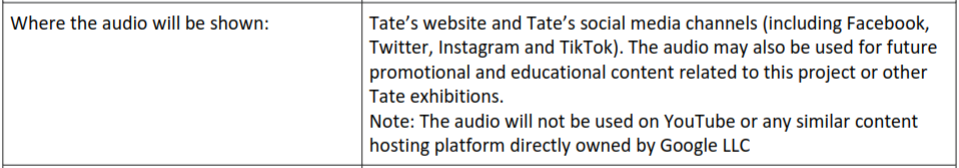
\includegraphics{media/lu3326961oku7t_tmp_a5eb5846ea3c9e21.png}
\caption{A screen shot from a contract between me and Tate displaying a
``Note'' disclaiming it cannot be shared on platforms run by Google
LLC}\label{fig:google}
}
\end{figure}

These inquiries into configure-able methods and configuring access aim
to give an insight into how crip studies and access-knowledge can
reconfigure configuration. They have set a basis to rethink how the
boundary between user/designer, requester/provider and body/institution
are delineated. In the de-sedimentation of delineation it moves us from
a need to cure the other or invalidate the frictions felt from
boundaries but instead care for how we can oriented towards and make
room for access to transform the sedimented inflexibility of
institutions. These methods orients to groups in context collectively
feeling out material relations and caring for their limits in a way that
generates unknowable possibilities. Each action of access an affirmation
of life, each affirmation a promise of a crip future to come.

\hypertarget{cripping-configuration}{%
\subsubsection{Cripping Configuration}\label{cripping-configuration}}

After returning to the crip table of critical access I want to return to
the genealogy of configuration to coalesce it close, inflect it with
-able and reorient it through these inquiries into configuring access.
In this moving from that of the straight axis of STS and towards a crip
queering of these methods. Part of this is to bring these methods
in-touch with the framework of this project, but also as mentioned is to
take up discourse of disability within feminist theory and configuration
management, where it has been present but unmentioned. The latter move
again informed by Kafer's work discussed in
\href{../02_Crip-Tic\%20of\%20vignettes/02.01.04_The\%20crip\%20table.md}{02.01.04\_The
crip table}, taking up disability in discourse where it is seen but not
felt. Again by cripping the axis of configuration, and disobediently
orienting it towards an abundance of crip futures, I am not discrediting
the great work of Suchman, but setting it to another background and in
reach of figures and practices of disability that can disorient its
sedimented norms. This disorienting of configuration for me is an action
of the internal arch's of this researcher's inquiry. It is to think
through how I relate to and practice organisational practices and theory
through my embodied knowledge's of crip methods and politics. It is also
for crip studies to make room for me to feel how these internal ripples
diffract, build up and make an impression and inflection on the path I
take towards and from configuration.

Here I reflect on the earlier two examples of configuration that Suchman
offers up to inflect their methods of critiquing the differences between
the prescribed plan and the situated actions of complex sociotechnical
systems, and in this how expertise are figured to roles and distributed.
The first thing that has to be noted here within her reflections of
these inquiries is the absence of disabled voices, theory and
experiences within this dialogues. Both clearly touch upon care systems,
whether they were experimental data management systems or the actioning
of metrified management of state care. Both of these case studies are
well within reach of crip politics and lives. On looking throughout the
paper the closest word to disability from a word search is fittingly
that of ``disappear'' within the scentence:

``In this sense, the method assemblage of configuration could be
understood as a device for articulating the relation between the
`insides' of a socio-technical system and its constitutive `outsides',
including all of those things that disappear in the system's figuration
as an object'' (Suchman 2012, 55)

This is not to say that Suchman is intentionally disappearing disabled
bodies and their experiences from configuring practices, but that the
norms of institutional logics place them as outsiders of their own
discourse. With Hamraie, I could also provocatively read this as
disabled practices of interdependence and embodied politics would
trouble the neutrality of this STS axis too much (2017, p.~50), so are
overruled to define a straight(er) line. Either reading, and the
situated actions of Suchman's definition have left disabled people
un-agential and disabled within dialogues of their own life giving
infrastructures. Below I take a closer reading of the two examples
Suchman offers to highlight how crip politics could disorient these
sedimented methods and wiggle them closer to my crip table and politics
of life affirmation.

With Ranjini's analysis of the ``Vision 2020'' scheme, Suchman's focus
on situated actions orients those of healthcare professionals in the
field. This scoping only shows how these people have to cut corners,
make up figures and hack metrics to maintain care within their
districts. This scoping, even though showing a clear separation between
plans of state management and situated actions of care on the ground,
does not make room for the people who had to be a corner that was cut.
Neither does it make room to highlight the violence that was enacted to
people in need of care when their district was punished for not hitting
targets and so given ill funding. In the silencing of disabled
experience here is the lack of a crip critique on these dynamics.

Here I aim to disorient these through both crip theories political
relational model's expansive critique of cure narratives that Kafer
offers (2013). In many ways the same methods of the medical model of
disability are also implicated to those working within the
infrastructure and organisation of healthcare in rural Andhra Pradesh,
southern India. In Ranjini's example the system was prescribed to be
cured of problems of inefficiencies by neo-liberal efficiency logics of
datafication and target hitting. This meant a few things, firstly that
the problem is isolated within the health care system and secondly the
``treatment'' given to cure it are data figure, metrics and targets.
This is apparent in Ranjini's notes, where even though acknowledged by
those having to hit them as semi-impossible in relation to the resources
provided and the situated material relations of people and space, those
figure, metrics and targets were still the only legitimate dialogue that
could be had. These organisational practices from ``district meetings
revealed no opportunity for health workers or supervisors to provide
explanations as to why targets could not be met, or to inform the
setting of more appropriate ones through''(Ibid, 54). And the efficient
logics inevitably led to penal systems where ``If they do not achieve
targets, they are punished. {[}Of course{]}, there is no reward. The
reward is not being punished.''(Ranjini 2007, 113). This system's
configuration turning to a treatment of a penal reward system similar to
that often used towards disabled people, from the ugly law through to
the eugenic persecution of ``feeble-minded'' (Kafer 2013, 30--32). These
penal logics also utalised by the AGI promises that I touch on in the
\href{../../00_Introduction/sections/00.01.00_Background.md}{00.01.00\_Background}
of the introduction. These are figure to promise to emerge generalised
intellignece and an ability to understand the unknown through automating
these same penal logics. Through a crip understanding of the
political/relational model though, these penal logics can be interpreted
as disabling any relation they are introduced into. They do this by
reducing the complex and nuanced relations of situated actions and
embodied practices that sociotechnical systems emerge from down to a
win/loose, valid/invalid equation. In doing so setting out a determinate
action space and reducing the metrics of success to singular goals that
are often unattainable within the material limits. The main issue my
crip critique has is how these logics disables the reading of any
alternative feedback or approach other than the desired unattainable
goals/metrics and by default not intimate with what it is being put in
touch with or impacting. Much like Ruha Benjamin's critique of
datafication of the injustice\footnote{``The datafication of injustice
  \ldots{} in which the hunt for more and more data is a barrier to
  acting on what we already know. We need something like an academic
  equivalent of ``I said what I said!'' -- the catchphrase of reality TV
  star NeNe Leakes -- for those who insist on digging deeper and deeper
  into the genome for scientific solutions to social problems.'' (R.
  Benjamin 2020, 117)}, and my own experiences of these dynamics at
\href{../02_Crip-Tic\%20of\%20vignettes/02.01.02_The\%20computing\%20table.md}{02.01.02\_The
computing table}, these systems and their policies prioritises data over
everything else. With an analysis of crip time we can also understand
this as gate-keeping needs from being met until the perfect data or cure
(that is unachievable) is achieved, and in the process invalidating,
irradicating and curing the unsqueezable bugs, temporary errors and ugly
data within the system.

The second example Suchman gives of Judith Gregory's analysis of the
HMO's experimental data management system, similarly frames disabled
people out of the dialogue. This is firstly through the works mapping of
the different groups figured to be valid voices within the development
of the data management system. Seemingly following the scoping set out
by the HMO, the only valid groups are the HMO, the technical developers
and the medical professionals. The closest they come to scoping in the
disabled experience of care and their opinion is through the patient's
data, which is figured to be ``always ready-to-hand''(Suchman 2012, 57).
Echoing my own experience of being ``cleen ready-to-use'' for
\href{../../02_Crip-Tic_of_Vignettes/sections/02.03_The_operating_table.md}{02.03\_The\_operating\_table},
this scoping misses the violence, objectification and industrialisation
of care that such an efficient imaginary entails. This forceful shaping
of the disabled bodies and patients into users in ready-to-use
configurations painfully emanates the eugenic histories the Hamraie
brings up with the flexible user (2017). This invalidation of voice and
experience undermines the scoping of this configuration's analysis, and
for me begs for crip disobedient intervention. It is a place for me to
refuse the expectation to be ``always ready-to-hand'' or ``cleen
reedy-to-use'', and instead step out of line and question how I can
situate plans and action from the sites of impact. In doing this giving
those at greatest risk as well as benefit, access to and agency over how
their infrastructures can affirm their current lives.

Searching for alternatives methods of configuration within Gregory's
critique of the HMO's Suchman highlights how Grgory takes up Helen
Verran's notion of ``working knowledges together''. In this notion
Verran is figuring out methods to bring together indigenous people and a
colonial state with very different imaginaries, capacities, practices
and their knowledges into other intermediary spaces for dialogue.
Gregory and Suchman highlight these indigenous land right discourses and
methods as a way to think through how to disorient the power relations
within plans, protocols and their negotiations. Verran's ``working
knowledges together'' is itself very interesting and has informed how I
approach discourse and power relations within my approach to collective
practices, but within the discourse of care systems it leaves me asking
for a little more. This is not to say that indigenous studies is not
applicable to disability discourse, it very much is in the ways that it,
along with other positionalities, multiplies the crip experiences as I
have mentioned in the
\href{../../01_Disability_justice_and_life_affirmation_flipping_the_table/sections/01.02.03_Crip_intersectionality.md}{01.02.03\_Crip\_intersectionality}
and
\href{../../01_Disability_justice_and_life_affirmation_flipping_the_table/sections/01.02.04_Cripping_Technoscience.md}{01.02.04\_Cripping\_Technoscience}
sections. Instead here specifically I wondered more why when they were
looking outside of the medical management discourse and to disorient it,
they didn't move to critical-access or disability studies? Why not turn
to Hamraie's critique of the flexible user (which wasn't written yet)?
or to Sins in-valid's intersectional collective practices? Of coalition
politics of disabled folks that go back decades? and of life affirming
access practices and their knowledges? Here when Suchman and Gregory
turn to the other outside of their western academic norms, they miss the
other being directly impacted by the system they are inquiring into.
With this -able inflection I aim to disorient the normative access of
STS that holds in place these bodily horizons through these determined
roles and invalidating relations. In doing this I not only start to
practice how crip theory and its methods, politics and practices can
disorient the norms, roles and divides of expertise in configuration
practices, but also how it makes room for configuration to feedback from
embodied collective practices, and ones that care for the sites of
impact within configurations.

Returning to Amoore's (2020) update of configuration, we can also
witness how in many ways she makes room for this distribution of roles
from the axis of user/designer, STS expert/practitioner,
prescriber/prescribed, to move to those of interdependent and collective
narrative making from the sites of impact and through many orientations,
approaches and capacities. In this though she still manages to negate
disability studies as being a place to pull from, instead turning to
almost every other marginalised group but disability\footnote{``It seems
  that the struggles of our contemporary moment --- resisting the rise
  of far-right nationalist groups, racist doctrines of anti-
  immigration, the everyday violences of sexism, racism, and bigotry ---
  confront also the profound difficulties of finding an opening at the
  limit of the frame. Indeed, many of our most important and difficult
  historical political struggles --- anti-apartheid movements, the civil
  rights movement, campaigns for lgbtq+ rights --- would arguably have
  been impeded by state access to algorithms that could learn to
  attribute future threats. In short, machine learning algorithms are
  actively making it more difficult for new ethicopolitical claims ---
  those claims not already registered as claimable --- to be made in the
  world. In this context, a cloud ethics must be able to locate ways of
  being together that resist the algorithmic forces 0f attribution.''
  (Amoore, 2020, p.~170)}. When we return to her work through critical
access and crip theory, we could understand partiality as capactiy, and
opacity as access. This transforms partiality, to be understood as a
relational materiality, where I practice within a technologies
capacities by configuring them out to understand, figure out and care
for their limits. It also refuses the boundary of opacity, aiming to not
conflate the sedimented roles and positions of configurations, but to
make room to figure out their interdependent relations and situated
processes. Crip studies and critical access here provide not only
another background to set these collective configuring methods from, but
in doing so re-figures the approaches configuration can take towards
complex sociotechnical systems and collective organisation.

\hypertarget{conclusion}{%
\subsection{Conclusion}\label{conclusion}}

This chapter in the thesis, is meant to hold an internal arc or
inflection that disorients both this researchers path and their use of
configuration as method. It inflects this research from inquiring into
the dialogues of centralised plans to instead orient toward
interdependent practices of configuring life affirming infrastructures
from site of impact. Through forming a genealogy of configuration, and
then inflecting it with a crip -able, I aim to have set a new background
to configure out the rest of this thesis inquiries from., and one that
centres places of impact and the design frictions that emerge in action.
In the next chapters I take these Configure-Able Methods into deeper
collective inquiries. In these inquiries I form a more nuanced and
situated understanding of what practising critical access across
multiple technical and social domains made know-able to collaborators
and I around our practices of collective configuration. In doing this I
aim to show how we can practice disability discourse not as a single
issue topic, or where we have to participate in or assimilate to
determinate dialogues, but instead centre critical access as a
generative place to improvise community infrastructures around and
configure interdependent life affirming futures from.
